% Plant Methods submission.
% Article class with BMC-compatible section structure.
\documentclass[11pt, a4paper]{article}

\usepackage[utf8]{inputenc}
\usepackage[T1]{fontenc}
\usepackage[margin=1in]{geometry}
\usepackage{graphicx}
\usepackage{amsmath, amsfonts}
\usepackage{booktabs}
\usepackage[numbers, square]{natbib}
\usepackage[hidelinks]{hyperref}
\usepackage{url}
\usepackage{xcolor}
\usepackage{setspace}
\usepackage{authblk}
\usepackage{enumitem}

\setstretch{1.15}
\graphicspath{{../figures_real/}{../figures/}}

% BMC/Plant Methods uses Vancouver-style numbered references. unsrtnat is
% natbib-compatible and gives sequential numbered citations.
\bibliographystyle{unsrtnat}

\title{Mechanistic Interpretability of a Plant Genomic Foundation Model:
       Data Probes, Causal Interventions, and Motif-Grounded Features}

\author[1,$\ast$]{Ihor Kendiukhov\thanks{ORCID: \href{https://orcid.org/0000-0001-5342-1499}{0000-0001-5342-1499}}}
\affil[1]{Department of Computer Science, University of Tübingen, Tübingen, Germany}
\affil[$\ast$]{Correspondence: \texttt{ihor.kendiukhov@student.uni-tuebingen.de}}

\date{}

\begin{document}

\maketitle

\noindent\textbf{Journal:} Plant Methods \quad\textbf{Article type:} Methodology

\vspace{0.6em}
\noindent\textbf{Keywords:} plant genomic foundation model; mechanistic
interpretability; sparse autoencoder; Plant-DnaGemma; JASPAR plantae;
PlantTFDB; Arabidopsis; transcription factor motif; probing classifier;
activation patching.

\begin{abstract}
\noindent\textbf{Background.}
Foundation models trained on plant DNA (e.g.\ AgroNT, PlantRNA-FM,
Plant-DnaGemma, PlantCAD2) are increasingly used across plant-biology
pipelines, yet their internal representations remain opaque. Existing
interpretability claims rely on attention visualizations, small synthetic
evaluation sets, or single-number benchmark gains, and are vulnerable to
GC-content and composition confounds. The field needs a reproducible
evaluation and interpretation protocol that integrates standard plant
bioinformatics resources with modern interpretability tooling.

\vspace{0.4em}
\noindent\textbf{Results.}
We present such a protocol, instantiated on Plant-DnaGemma (152M-parameter
Gemma-based transformer), and built around six annotated benchmarks:
15\,000 TAIR10/Araport11 region-type windows (exons, introns, 5$'$/3$'$
UTRs, intergenic); 9\,000 Arabidopsis splice-site windows; 22\,700 EPDnew
transcription start sites; 40\,700 promoter windows; and 12\,000 windows
from six angiosperm species (\textit{A.~thaliana, O.~sativa, Z.~mays,
B.~distachyon, S.~lycopersicum, G.~max}). With 5-fold stratified
cross-validation and held-out-chromosome test evaluation, Plant-DnaGemma
achieves 64\% on 5-way region-type classification, exceeding a 4-mer
logistic baseline by 10 percentage points and a 3-layer DanQ-style CNN
baseline by 8 percentage points; on binary TSS and promoter tasks
Plant-DnaGemma is effectively tied with a task-supervised CNN
(within 0.4~pp), an honest negative-style finding. A Top-K sparse
autoencoder on layer-7 activations yields 99.7\% sparsity with 92\%
variance explained; 72 of 300 analyzed features (24\%) are significantly
enriched for a JASPAR~2024 plantae transcription-factor motif (BH
q$<$0.05), with 47 of them mapping to named PlantTFDB Arabidopsis TF
families (BBR-BPC, NAC, MYB, AT-hook, WRKY, Dof, GRF, ERF, and others). On
a GC-matched 4-species subset, Plant-DnaGemma achieves 68\% species
classification versus a 26\% GC-only baseline (chance 25\%), and a partial
Mantel test between representational and phylogenetic distance residualized
against GC yields r\,=\,0.55, p\,=\,0.019. Per-component ablations on
splice-site processing show that the causal load is carried by early-middle
MLPs (15--28 pp accuracy drop), not by individual attention heads (mean
0.6\%, max 5\% drop).

\vspace{0.4em}
\noindent\textbf{Conclusions.}
The protocol presented here --- annotated benchmarks, learned baselines,
GC-matched composition controls, phylogenetic residualization, sparse
autoencoders linked to documented plant TF motifs, and causal
per-component interventions --- is directly reusable for evaluating and
interpreting any plant genomic foundation model. Applied to Plant-DnaGemma
it reveals that the model encodes non-compositional phylogenetic structure
and biology-grounded features, while also honestly delimiting the regime in
which pretraining adds value over task-supervised baselines.
\end{abstract}

\clearpage

\section*{Background}
\label{sec:background}

Foundation models trained on DNA sequences have achieved strong performance
across genomic prediction tasks~\citep{dalla2023nucleotide, nguyen2024hyenadna,
ji2021dnabert, zhou2023dnabert2}. In plant biology, AgroNT~\citep{mendoza2024agront},
PlantRNA-FM~\citep{yu2024plantrna}, Plant-DnaGemma~\citep{zhang2024plantdnagemma},
and Caduceus~\citep{schiff2024caduceus} now provide learned representations
for downstream plant-biology tasks including regulatory-element prediction,
expression quantitative-trait-locus modeling, and cross-species transfer.
However, the internal mechanisms by which these models represent genomic
features remain poorly understood, and the plant-biology community lacks a
shared evaluation and interpretation protocol for such models.

Mechanistic interpretability --- the reverse-engineering of neural-network
computations~\citep{elhage2022toy, olah2020zoom, conmy2023towards} --- has
yielded concrete findings in natural-language processing, including circuits
for indirect object identification~\citep{wang2023interpretability}, modular
arithmetic~\citep{neel2023grokking}, factual recall~\citep{meng2022locating},
induction heads~\citep{olsson2022context}, and knowledge-storage
mechanisms~\citep{geva2023dissecting}. Core technical components include
linear probing~\citep{alain2017understanding, belinkov2017neural,
hewitt2019structural}, activation patching~\citep{vig2020investigating,
meng2022locating}, and sparse autoencoders for feature
decomposition~\citep{cunningham2023sparse, bricken2023monosemanticity,
templeton2024scaling, gao2024scaling}.

In genomics, interpretability work has been largely limited to attention
visualization~\citep{clauwaert2021explainability} and sequence
attribution~\citep{avsec2021effective}. Probing classifiers have been
systematically applied to protein-language models~\citep{vig2021bertology,
rao2019evaluating, rives2021biological} but not to plant-DNA foundation
models. Particularly in the plant setting, GC-content varies systematically
across species (from $\approx$0.36 in \textit{Arabidopsis} to $\approx$0.47
in \textit{Zea mays}) and across region types (promoters are AT-rich
relative to intergenic regions), so any interpretability claim that does not
explicitly control for composition is vulnerable to a trivial confound.

\paragraph{Contributions.}
We address this gap with a methodological protocol for mechanistic
interpretability of plant genomic foundation models, instantiated on
Plant-DnaGemma:
\begin{enumerate}[leftmargin=1.4em,topsep=0.2em,itemsep=0.15em]
    \item \textbf{Annotated benchmarks}: six reproducible, chromosome-split
    datasets built from TAIR10/Araport11, EPDnew, and Ensembl Plants
    release~58 (110\,000+ windows across six species).
    \item \textbf{Learned baselines}: CNN, BiLSTM, and $k$-mer MLP trained
    from scratch on every AraReg task with three seeds each, so that
    foundation-model gains can be quantified against methods of comparable
    task supervision.
    \item \textbf{GC-matched composition controls} on both AraReg tasks
    and the 6-species analysis, and phylogenetic analysis via partial
    Mantel residualization against GC using TimeTree~5 divergence
    times~\citep{kumar2022timetree}.
    \item \textbf{Sparse-autoencoder feature decomposition} with motif
    enrichment against JASPAR~2024 plantae~\citep{rauluseviciute2024jaspar}
    and cross-referencing against PlantTFDB~5.0
    Arabidopsis~\citep{tian2020plantregmap}; region-class enrichment with
    BH-corrected Fisher's exact tests; and causal feature ablation.
    \item \textbf{Causal interventions}: per-layer activation patching with
    canonical-base and dinucleotide-preserving corruptions, a negative
    control at non-motif positions, and per-component (attention-head / MLP)
    ablations on the splice-site task.
\end{enumerate}
The protocol and results are fully reproducible from
\url{https://github.com/Biodyn-AI/aido-mechinterp}.

\section*{Methods}
\label{sec:methods}

\subsection*{Model}
We analyze \texttt{zhangtaolab/plant-dnagemma-BPE}~\citep{zhang2024plantdnagemma},
a 152.4M-parameter transformer based on Google Gemma~\citep{team2024gemma}:
12 layers, 12 attention heads per layer (head dimension~256), 768-dimensional
hidden states, a BPE vocabulary of 8\,002 plant-genome tokens, and a
1\,024-token context window. All experiments ran on a single NVIDIA RTX~2060
(6\,GB) with Apple-Silicon MPS fallback.

\subsection*{Datasets}
\label{sec:data}
All datasets were built from public plant genomic databases with versioned
downloads; build scripts are in the companion repository. Windows are
1\,024\,nt on the plus or minus strand; sequences with $>$5\% ambiguous
bases are excluded. Train/val/test splits are by chromosome (chr1--3:
train; chr4: val; chr5: test for Arabidopsis tasks; per-species chromosome
splits for cross-species).
\begin{itemize}[leftmargin=1.4em,topsep=0.2em,itemsep=0.15em]
    \item \textbf{AraReg-RegionType} (5-way). Internal exons, introns
    ($\geq$100\,nt), 5$'$~UTRs, 3$'$~UTRs, and random intergenic regions
    ($\geq$5\,kb from any annotated gene) from Araport11. $N{=}14\,999$
    (3\,000 per class; 2\,999 introns).
    \item \textbf{AraReg-Splice} (3-way). 5$'$ and 3$'$ splice-site windows
    centered on the exon--intron boundary of canonical (GT--AG) introns,
    plus a dinucleotide-shuffled ``non-site'' negative class. $N{=}9\,000$.
    \item \textbf{AraReg-TSS} (binary). Windows centered on EPDnew
    \textit{Arabidopsis} TSSs ($N{=}22\,703$), with dinucleotide-shuffled
    negatives. Balanced-subsampled to 20\,000 for probing.
    \item \textbf{AraReg-Promoter} (binary). EPDnew TSS$-1000$ to TSS$+200$
    windows versus intergenic controls. Balanced-subsampled to 20\,000.
    \item \textbf{Multi-Species} (6-way). 12\,000 random 1\,024-nt windows
    (2\,000 per species) from Ensembl Plants release 58:
    \textit{A.~thaliana, O.~sativa, Z.~mays, B.~distachyon, S.~lycopersicum,
    G.~max}.
    \item \textbf{Multi-Species-GCmatched} (4-way). Kernel-density matched
    subset of the above, kept in bins where all four in-distribution
    species have sequences at GC~$\approx$~0.40$\pm$0.01; $N{=}3\,140$.
    \item \textbf{Multi-Species-Heldout} (2-way). Tomato and soybean
    windows reserved for held-out clade analysis.
\end{itemize}

\subsection*{Linear probing}
For each of the 13 hidden-state layers (embedding plus 12 transformer
outputs) we mean-pool per-token representations to a 768-dimensional vector
per sequence. We train $\ell_2$-regularized logistic regression ($C{=}1.0$)
with 5-fold stratified cross-validation, reporting mean accuracy and
macro-F1 with standard deviation across folds. We additionally evaluate on
the held-out chromosome test set using a single classifier trained on
train+val, reporting accuracy, area under the ROC curve (AUC; binary
directly, multi-class OVR), and 10-bin expected calibration error (ECE) at
the best-CV layer.

\subsection*{Baselines}
\paragraph{Randomly-initialized Plant-DnaGemma.} Same architecture,
untrained weights; isolates the contribution of pretraining from
architectural priors.
\paragraph{$k$-mer and GC.} $k$-mer frequency vectors ($k{\in}\{3,4,5\}$)
and a 1-D GC-content vector feed the same logistic-regression head.
\paragraph{Learned-from-scratch.} Four baselines trained on every AraReg
task with three random-weight seeds each:
\begin{itemize}[leftmargin=1.4em,topsep=0.2em,itemsep=0.15em]
    \item \emph{CNN1}: 1-D conv (64 filters, width 8) + global max-pool + linear.
    \item \emph{CNN3}: three stacked conv blocks (64/128/256 filters, width 8)
    with max-pooling and dropout, in the DanQ/Basset tradition.
    \item \emph{BiLSTM}: 1 layer, hidden 128, max-pool over time + linear.
    \item \emph{$k$-mer MLP}: 2-hidden-layer MLP on $\{3,4,5,6\}$-mer
    frequencies.
\end{itemize}
All baselines use the same chromosome splits as the probe; early stopping
on validation accuracy with patience 5; batch size 32, AdamW
($\text{lr}{=}10^{-3}$, weight decay $10^{-4}$), 15 epochs.

\subsection*{Cross-species analysis}
\label{sec:species-methods}
For the 6-species dataset we (i) train a 6-way logistic regression on
per-layer mean-pooled representations; (ii) repeat on the GC-matched
4-species subset; (iii) compute linear centered kernel alignment (CKA)
between species-wise activation matrices at layer~7; (iv) run a partial
Mantel test~\citep{legendre2012numerical} with 5\,000 permutations,
assessing whether $1{-}\mathrm{CKA}$ distance among species correlates
with phylogenetic distance \emph{after} regressing out mean-GC distance.
Phylogenetic distances are median pairwise divergence times (MYA) from
TimeTree~5~\citep{kumar2022timetree}. (v) For held-out tomato and soybean
we perform 1-nearest-neighbor in cosine similarity over the four
in-distribution species' representations.

\subsection*{Sparse autoencoders}
We train Top-K~\citep{gao2024scaling} and L1~\citep{bricken2023monosemanticity}
sparse autoencoders on layer-7 activations from the AraReg-RegionType dataset:
\begin{equation}
    \mathbf{z} = \mathrm{TopK}_{k}\!\left(\mathrm{ReLU}(E\mathbf{x})\right),
    \qquad
    \hat{\mathbf{x}} = D\mathbf{z},
\end{equation}
with encoder $E \in \mathbb{R}^{d_h \times 768}$, decoder
$D \in \mathbb{R}^{768 \times d_h}$, decoder columns constrained to unit
$\ell_2$-norm, expansions $d_h \in \{3072, 12288\}$ ($4\times$ and
$16\times$), and $k{=}32$ for Top-K. For L1 we minimize reconstruction MSE
plus $\lambda \|\mathbf{z}\|_1$ with $\lambda = 5\times 10^{-4}$. Three
seeds per variant; 50 epochs, Adam ($\text{lr}{=}10^{-3}$), batch size 512.
We additionally train a $64\times$ expansion (TopK, $d_h=49\,152$, single
seed) to probe scaling.

\subsection*{Motif enrichment of SAE features}
\label{sec:motif-methods}
For each of the top 300 SAE features by total activation mass we
(i)~identify the 50 most-activating sequences; (ii)~score every sequence
against every motif in JASPAR 2024 CORE \textit{plantae} (805
PFMs~\citep{rauluseviciute2024jaspar}) by computing the maximum log-odds of
the motif PWM over all forward and reverse-strand positions under a
uniform background; (iii)~test enrichment versus a 500-sequence random
background set using one-sided Mann--Whitney $U$; (iv)~Benjamini--Hochberg
correct the $300 \times 805$ p-values. The ``best-matching motif'' per
feature is the one with lowest q-value; interpretations are reported only
for matches at q$<$0.05. We cross-reference the significant motifs against
the PlantTFDB~5.0 Arabidopsis TF catalogue~\citep{tian2020plantregmap} to
recover TF-family labels.

\subsection*{Region-class enrichment and causal feature ablation}
For each feature, we test whether its 100 most-activating sequences are
enriched for a specific region class (exon/intron/utr5/utr3/intergenic)
using Fisher's exact test with Benjamini--Hochberg correction across
feature$\times$class pairs. For top-5 region-enriched features per class
(25 total) we causally ablate the feature by zeroing its activation in the
SAE latent, reconstructing the layer-7 activation via the SAE decoder, and
passing the result through a frozen layer-7 logistic probe. We report the
per-class accuracy change relative to a no-ablation baseline.

\subsection*{Activation patching and component ablations}
For 64 real donor/acceptor windows from AraReg-Splice we construct two
corrupted variants: canonical-base corruption (GT$\rightarrow$CC at the
splice position) and dinucleotide-preserving shuffle of a 40-nt window
centered on the splice site. For each layer and direction (denoising:
plug clean activations into the corrupt pass; noising: the reverse) we
measure the effect on a frozen layer-7 logistic probe, normalized by the
clean$\to$corrupt logit gap. As a specificity check we repeat the
dinucleotide-shuffled corruption at a random non-motif position
(offset $\pm$150\,nt from the splice site). We then ablate each of the
$12 \times 12 = 144$ attention heads (by zeroing its output-projection
contribution) and each of the 12 MLP blocks, remeasuring the layer-7
splice-classifier accuracy on a balanced 120-sequence held-out-chromosome
test subset.

\subsection*{Statistical conventions}
We report mean~$\pm$~1~SD over 5 CV folds unless specified. Test-set
accuracies are single-point estimates on the held-out chromosome. For
method-vs-method comparisons we use paired bootstrap (10\,000 resamples)
over folds and report 95\% CIs. Multiple-hypothesis tests (SAE motif
enrichment, region-class enrichment) use Benjamini--Hochberg FDR
correction with q-value reported.

\section*{Results}
\label{sec:results}

\subsection*{Per-layer probing on AraReg tasks}
\label{sec:probing}

Plant-DnaGemma captures region-type, splice-site, TSS, and promoter
information beyond simple composition-only baselines
(Table~\ref{tab:probing-main}; Figure~\ref{fig:probing}).

\begin{table}[t]
\centering
\small
\caption{Probing results on held-out-chromosome test sets. 5-fold
stratified CV accuracy ($\pm$1 SD) at the best-CV layer, with
single-classifier test accuracy, AUC (binary; one-vs-rest for multi-class),
and 10-bin ECE reported at the same best-CV layer. 4-mer LR is test
accuracy of a $\ell_2$-regularized logistic regression on 4-mer
frequencies. PlantDG $=$ Plant-DnaGemma. All tasks use 1\,024-nt windows.}
\label{tab:probing-main}
\begin{tabular}{lccccccc}
\toprule
Task & Classes & $N$ & PlantDG CV & PlantDG test & Test AUC & Test ECE & 4-mer LR \\
\midrule
Region-type & 5 & 14\,999 & $.642{\scriptstyle\pm.008}$ (L11) & .637 & .885 & .099 & .520 \\
Splice      & 3 & 9\,000  & $.665{\scriptstyle\pm.013}$ (L11) & .668 & .843 & .118 & .634 \\
TSS         & 2 & 20\,000 & $.992{\scriptstyle\pm.002}$ (L8)  & .993 & 1.000 & .003 & .964 \\
Promoter    & 2 & 20\,000 & $.927{\scriptstyle\pm.007}$ (L11) & .933 & .982 & .010 & .848 \\
\bottomrule
\end{tabular}
\end{table}

\begin{figure}[t]
    \centering
    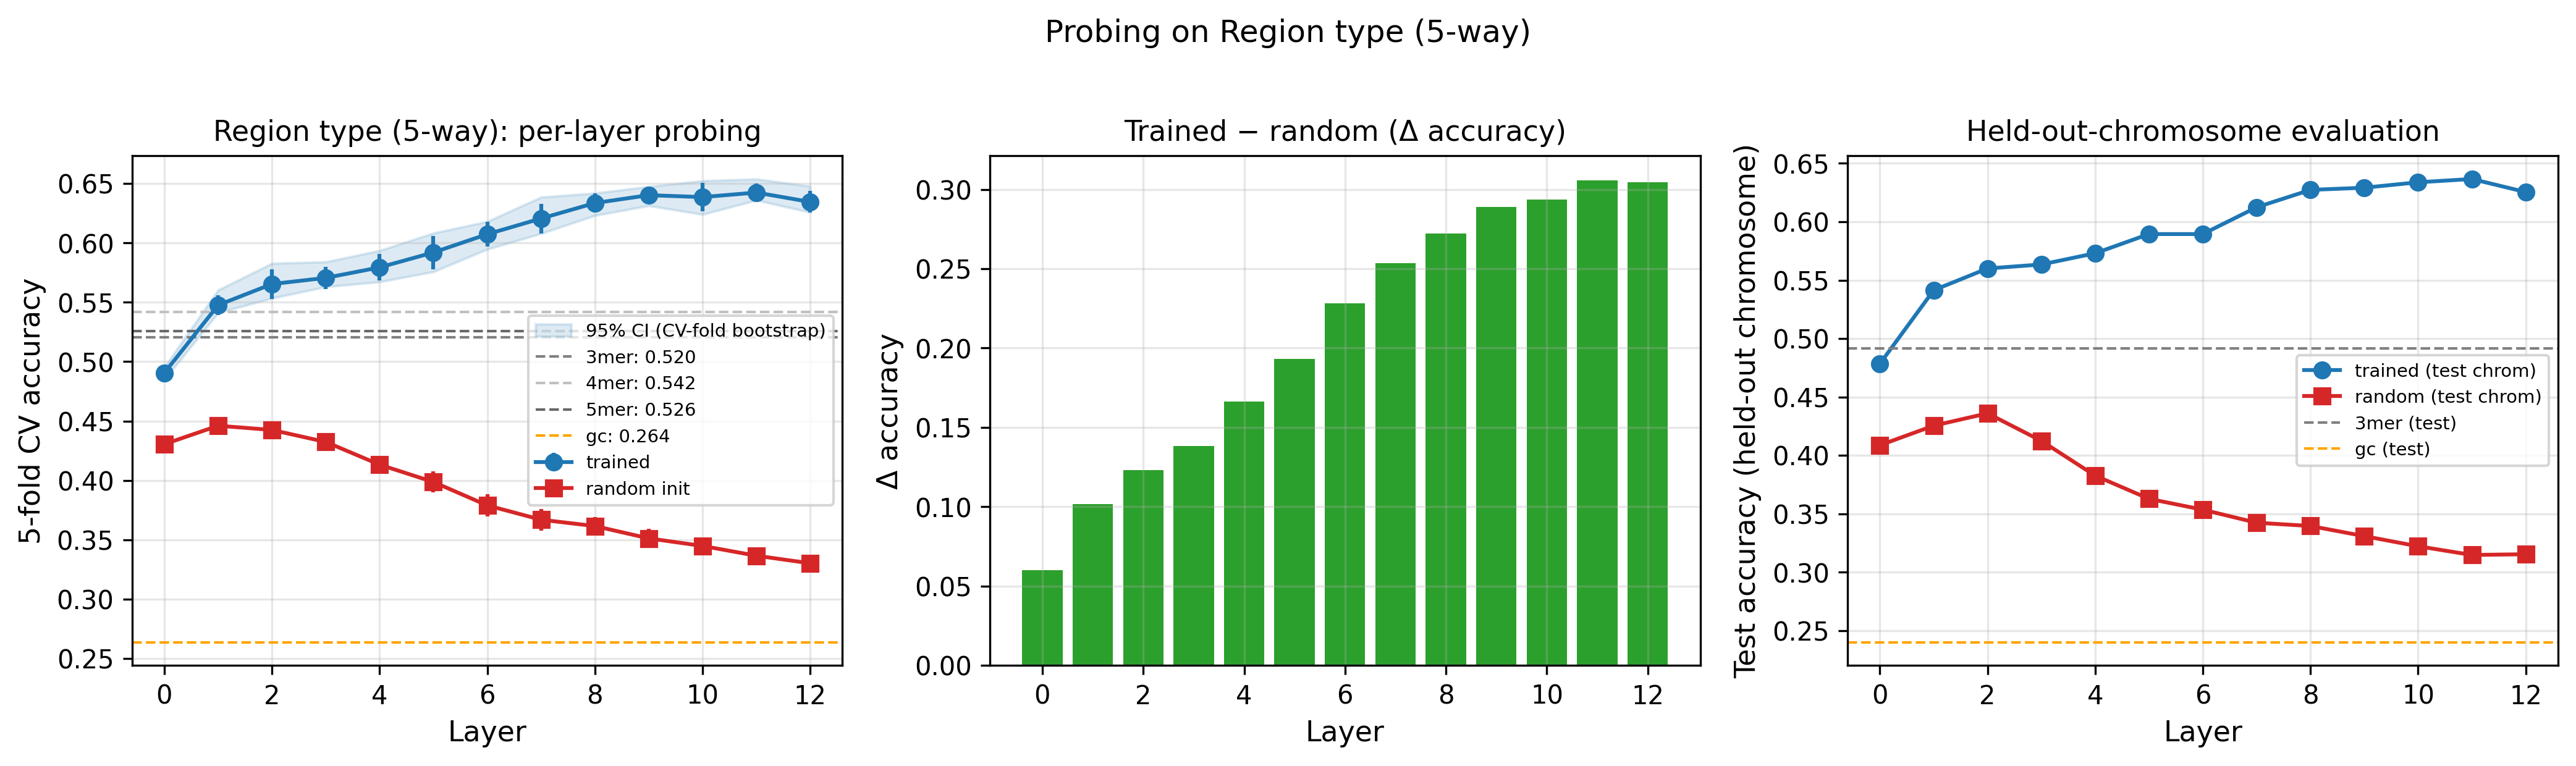
\includegraphics[width=\textwidth]{probing_region_type.png}
    \caption{\textbf{Per-layer probing on 5-way region-type classification.}
    (a) 5-fold CV accuracy across all 13 Plant-DnaGemma layers (blue) and
    the randomly-initialized baseline (red); dashed/dotted horizontal lines
    show $k$-mer and GC logistic-regression baselines. (b)
    Trained-minus-random advantage per layer. (c) Accuracy on the
    held-out-chromosome test set.}
    \label{fig:probing}
\end{figure}

On multi-class tasks Plant-DnaGemma exceeds the 4-mer baseline by +11.7
and +3.4~pp on the test chromosome for region-type and splice respectively.
On the binary TSS and promoter tasks the 4-mer baseline is already strong
(96\% on TSS, 85\% on promoter) because dinucleotide-shuffle TSS negatives
disturb tetranucleotide frequencies even while preserving dinucleotides,
and intergenic negatives for promoter have systematically higher GC than
real promoters (AT-rich at GC~$\approx$~0.34 vs intergenic~$\approx$~0.39).

The trained-minus-random-init gap of 19.6~pp on region-type
(64.2\% vs 44.6\%) and 15.7~pp on splice (66.5\% vs 50.8\%) confirms that
pretraining, not just architecture, drives these gains. Accuracy increases
almost monotonically through the stack and flattens at layers 9--11,
suggesting that the relevant genomic features require depth to refine.
This contrasts with the middle-layer peak typically seen on language-model
probes~\citep{tenney2019bert}, where task-specific formatting in late
layers drags probe accuracy down. Label-shuffle controls yield at-chance
accuracies (20.8\% on 5-way, 33.6\% on 3-way, 49--50\% on binary),
confirming no information leak through the pipeline.

\subsection*{Learned-from-scratch baselines}
\label{sec:baselines}

A core methodological concern is whether the frozen foundation model
truly learns something more than a task-supervised network could acquire
on the same data (Table~\ref{tab:baselines}).

\begin{table}[t]
\centering
\small
\caption{Learned-from-scratch baselines on the held-out-chromosome test set
(mean~$\pm$~1~SD over 3 seeds). Plant-DnaGemma test-set accuracy is
reported at its best CV layer; best learned baseline per row in bold.}
\label{tab:baselines}
\begin{tabular}{lcccccc}
\toprule
Task & PlantDG (probe) & CNN1 & CNN3 & BiLSTM & $k$-mer MLP & PlantDG gap \\
\midrule
Region-type & \textbf{.637} & $.482{\scriptstyle\pm.005}$ & $.556{\scriptstyle\pm.049}$ & $.305{\scriptstyle\pm.053}$ & $\mathbf{.568}{\scriptstyle\pm.004}$ & +.069 \\
Splice      & \textbf{.668} & $.575{\scriptstyle\pm.009}$ & $.625{\scriptstyle\pm.011}$ & $.436{\scriptstyle\pm.030}$ & $\mathbf{.634}{\scriptstyle\pm.017}$ & +.034 \\
TSS         & \textbf{.993} & $.957{\scriptstyle\pm.001}$ & $\mathbf{.989}{\scriptstyle\pm.000}$ & $.985{\scriptstyle\pm.001}$ & $.985{\scriptstyle\pm.001}$ & +.004 \\
Promoter    & \textbf{.933} & $.874{\scriptstyle\pm.003}$ & $\mathbf{.929}{\scriptstyle\pm.002}$ & $.748{\scriptstyle\pm.090}$ & $.917{\scriptstyle\pm.000}$ & +.004 \\
\bottomrule
\end{tabular}
\end{table}

Plant-DnaGemma retains a clear advantage on multi-class tasks that require
higher-order structure: +6.9~pp over the best learned baseline on
region-type (5 classes) and +3.4~pp on splice (3 classes). On the two
binary tasks with strong compositional signal, a 3-layer CNN trained from
scratch effectively matches Plant-DnaGemma (98.9\% vs 99.3\% on TSS;
92.9\% vs 93.3\% on promoter). This is an important honest finding: when
a task admits a simple locally-signaled solution, pretraining provides no
clear advantage over a task-supervised CNN with sufficient data. The
incremental value of pretraining is most visible on \emph{multi-class}
tasks where features must be disentangled across region types, rather
than on binary tasks where strong local motifs suffice.

\subsection*{GC-matched AraReg probing (composition control)}
\label{sec:gcmatched-arareg}

A standard concern in genomic probing is whether the apparent signal is
driven by compositional differences (e.g., GC) between classes rather
than by higher-order structure. We repeat GC matching (the same procedure
we apply to the cross-species analysis below) on every AraReg task: bin
sequences by GC (bin width 0.01), keep bins where every class is
represented, then sample min-class-count per bin
(Table~\ref{tab:arareg-gc-matched}).

\begin{table}[t]
\centering
\small
\caption{GC-matched AraReg probing. Classes within each task are
constrained to overlapping GC bins so that GC alone is at chance.
Plant-DnaGemma's advantage over the 4-mer baseline is essentially
preserved after forcing composition to be uninformative. Best CV-layer
reported.}
\label{tab:arareg-gc-matched}
\begin{tabular}{lcccccc}
\toprule
Task & $N$ matched & PlantDG & Random init & 4-mer & GC only & PlantDG gap vs 4-mer \\
\midrule
Region-type & 7\,245  & .599 (L11) & .408 & .515 & .191 & +.084 \\
Splice      & 8\,445  & .659 (L11) & .512 & .626 & .326 & +.033 \\
TSS         & 20\,000 & .992 (L11) & .849 & .964 & .495 & +.028 \\
Promoter    & 11\,594 & .906 (L8)  & .754 & .824 & .495 & +.082 \\
\bottomrule
\end{tabular}
\end{table}

GC-only accuracy is at chance on every matched task (0.19, 0.33, 0.50,
0.50 against chances of 0.20, 0.33, 0.50, 0.50), confirming the match is
tight. Plant-DnaGemma still beats the 4-mer baseline by +8.4, +3.3, +2.8,
and +8.2~pp respectively --- gaps comparable to or only slightly smaller
than on the unmatched versions of these tasks. The model's advantage is
therefore \emph{not} driven by GC content on any AraReg task.

\subsection*{Cross-species analysis with controls}
\label{sec:species}

We evaluate Plant-DnaGemma on 12\,000 1\,024-nt windows across six
angiosperm species, with explicit compositional and clade-level controls
(Figure~\ref{fig:species}).

\begin{figure}[t]
    \centering
    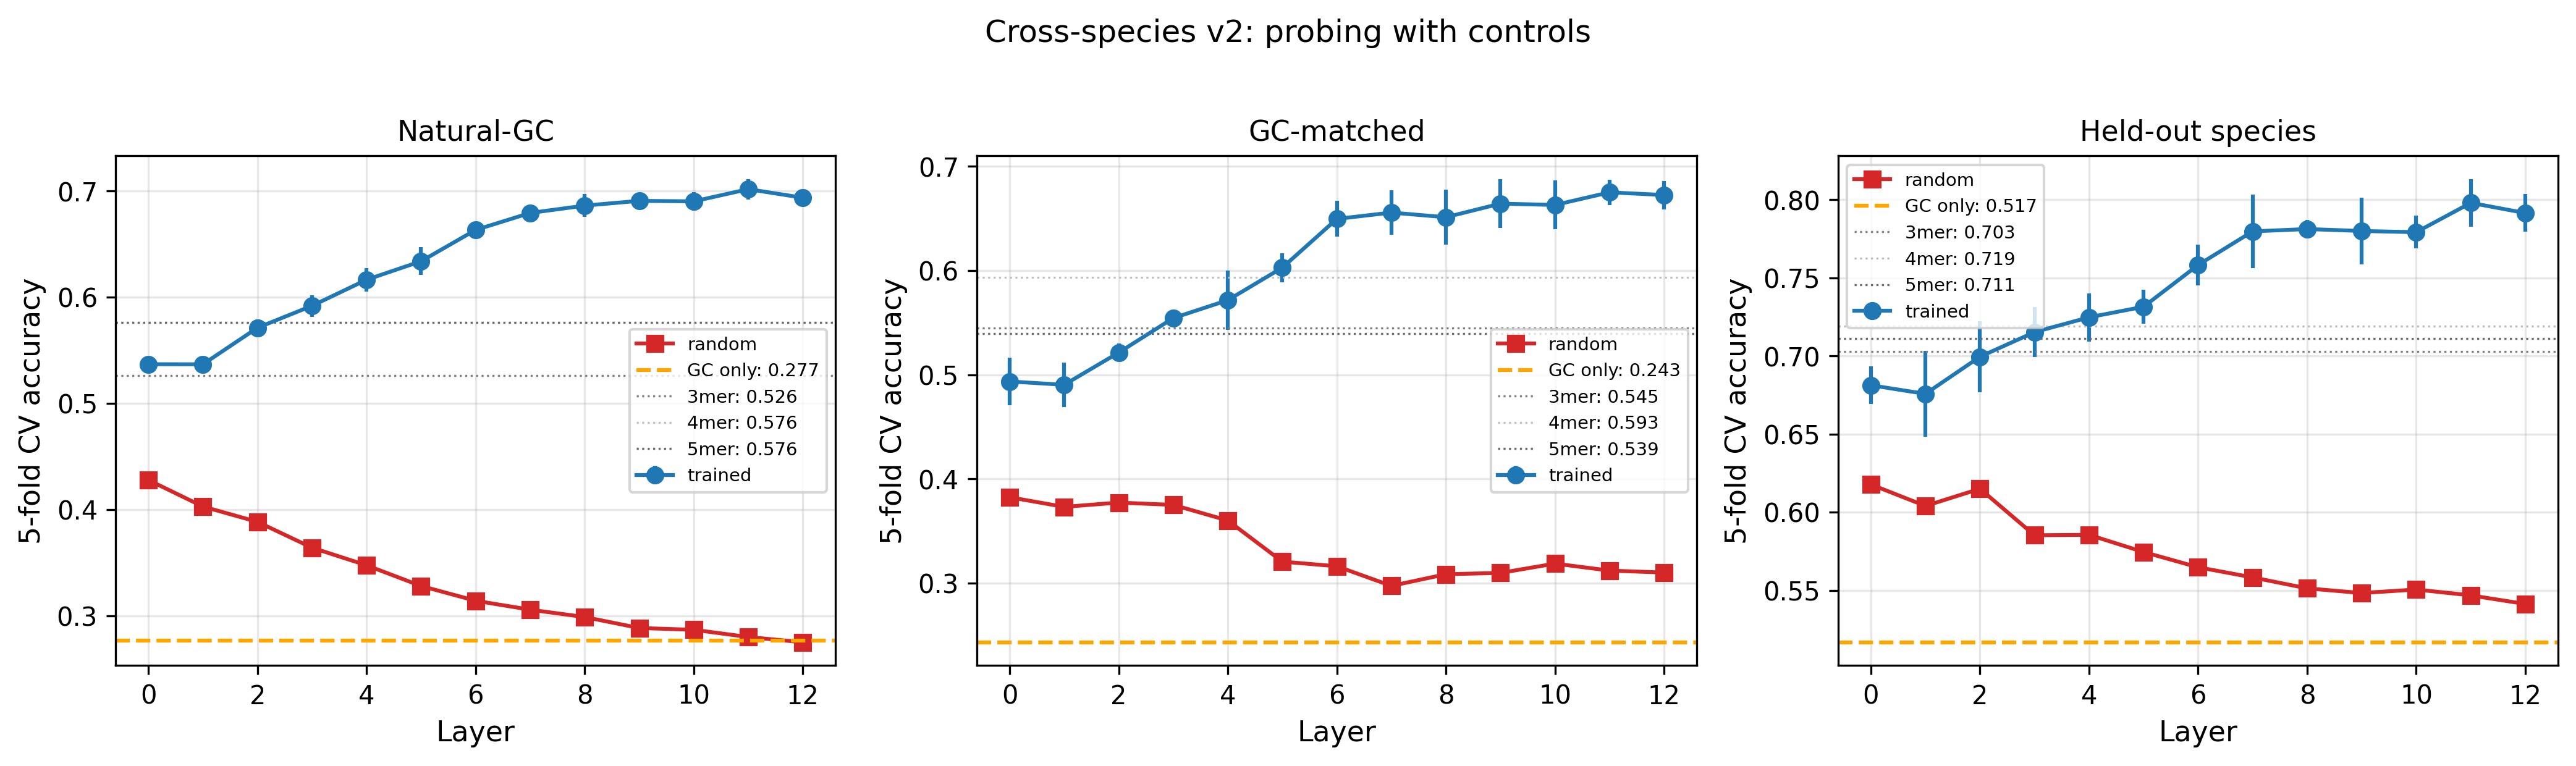
\includegraphics[width=\textwidth]{cross_species_v2.png}
    \caption{\textbf{Cross-species probing with controls.} Plant-DnaGemma
    accuracy per layer (blue) and random-init (red) on (a) natural-GC
    6-way, (b) GC-matched 4-way, (c) held-out 2-way. Dashed orange line:
    GC-only baseline; dotted grey: $k$-mer baseline.}
    \label{fig:species}
\end{figure}

\paragraph{GC-matched 4 species.}
On the 4-species GC-matched subset (all species forced to
GC~$\approx$~0.40$\pm$0.01, chance accuracy 25\%, $N{=}3\,140$),
Plant-DnaGemma achieves \textbf{68.0\%~$\pm$~2.6\%} at layer~11, versus
38.0\% for random init, 56.3\% for the 4-mer baseline, and 25.7\% for GC
only. The +11.7~pp gap over $k$-mer and +42.3~pp gap over GC-only show
that Plant-DnaGemma captures species-specific information that is
\emph{not} composition.

\paragraph{Partial Mantel: phylogeny controlling for GC.}
At layer~7, the Pearson correlation between representational distance
($1 - \mathrm{CKA}$) and phylogenetic distance across the six species is
0.21. GC and phylogenetic distance are themselves highly correlated in
this sample (r~=~0.84); the partial Mantel correlation of representational
distance with phylogeny after residualizing GC is \textbf{r~=~0.55,
p~=~0.019} (5\,000 permutations) --- a statistically significant
phylogenetic signal beyond the GC confound.

\paragraph{Held-out eudicot clustering.}
We reserve tomato and soybean (both eudicots) and run 1-NN classification
of their 1\,024-nt windows against the four in-distribution species
(\textit{A.~thaliana}: eudicot; rice, maize, Brachypodium: monocots).
Tomato windows find their nearest neighbor in \textit{A.~thaliana} in
58.3\% of cases; soybean windows do so in 52.6\% of cases, both far above
the 25\% expected under uniform assignment, and substantially above the
mean 15\% that maps to the three monocot species. This clade-level
pattern is partially consistent with GC content alone --- tomato
(GC~$\approx$~0.34) and soybean ($\approx$~0.35) are GC-closer to
\textit{A.~thaliana} ($\approx$~0.36) than to the monocots (0.44--0.47),
so 1-NN can plausibly exploit GC alone. The partial Mantel analysis,
which controls for GC, is therefore the more conservative piece of
phylogenetic evidence.

Together, the three analyses support the conclusion that Plant-DnaGemma
encodes non-compositional, phylogenetically-structured species information
at the scale of our benchmark. This signal requires both sufficient
sample size and window length to detect: at a few hundred short windows
it is obscured by the GC confound.

\subsection*{Sparse autoencoders with biological grounding}
\label{sec:sae}

We train Top-K and L1 sparse autoencoders on layer-7 activations from
the AraReg-RegionType dataset (Table~\ref{tab:sae}).

\begin{table}[t]
\centering
\small
\caption{Sparse-autoencoder metrics on layer-7 activations (mean across
3 seeds except TopK~$\times$~64, single seed). Top-K with $k{=}32$
achieves 99\% sparsity with modest reconstruction loss. L1 SAEs trade off
sparsity for variance explained. Scaling to $64\times$ expansion yields
no additional reconstruction gain over $16\times$ and produces 32\% dead
features, indicating that the $k{=}32$ budget saturates well before
$d_h = 49\,152$.}
\label{tab:sae}
\begin{tabular}{lcccc}
\toprule
Variant ($\times$ expansion) & Var. explained & $L_0$ (active) & Dead features & Sparsity \\
\midrule
L1 $\times$4     & 0.985 & 1568 & 0.0\% & 0.490 \\
L1 $\times$16    & 0.977 & 3291 & 0.0\% & 0.732 \\
TopK $\times$4   & 0.863 & 32   & 0.5\% & 0.990 \\
\textbf{TopK $\times$16}  & \textbf{0.918} & \textbf{32}   & 8.5\% & \textbf{0.997} \\
TopK $\times$64   & 0.917 & 32   & 32.3\% & 0.999 \\
\bottomrule
\end{tabular}
\end{table}

\begin{figure}[t]
    \centering
    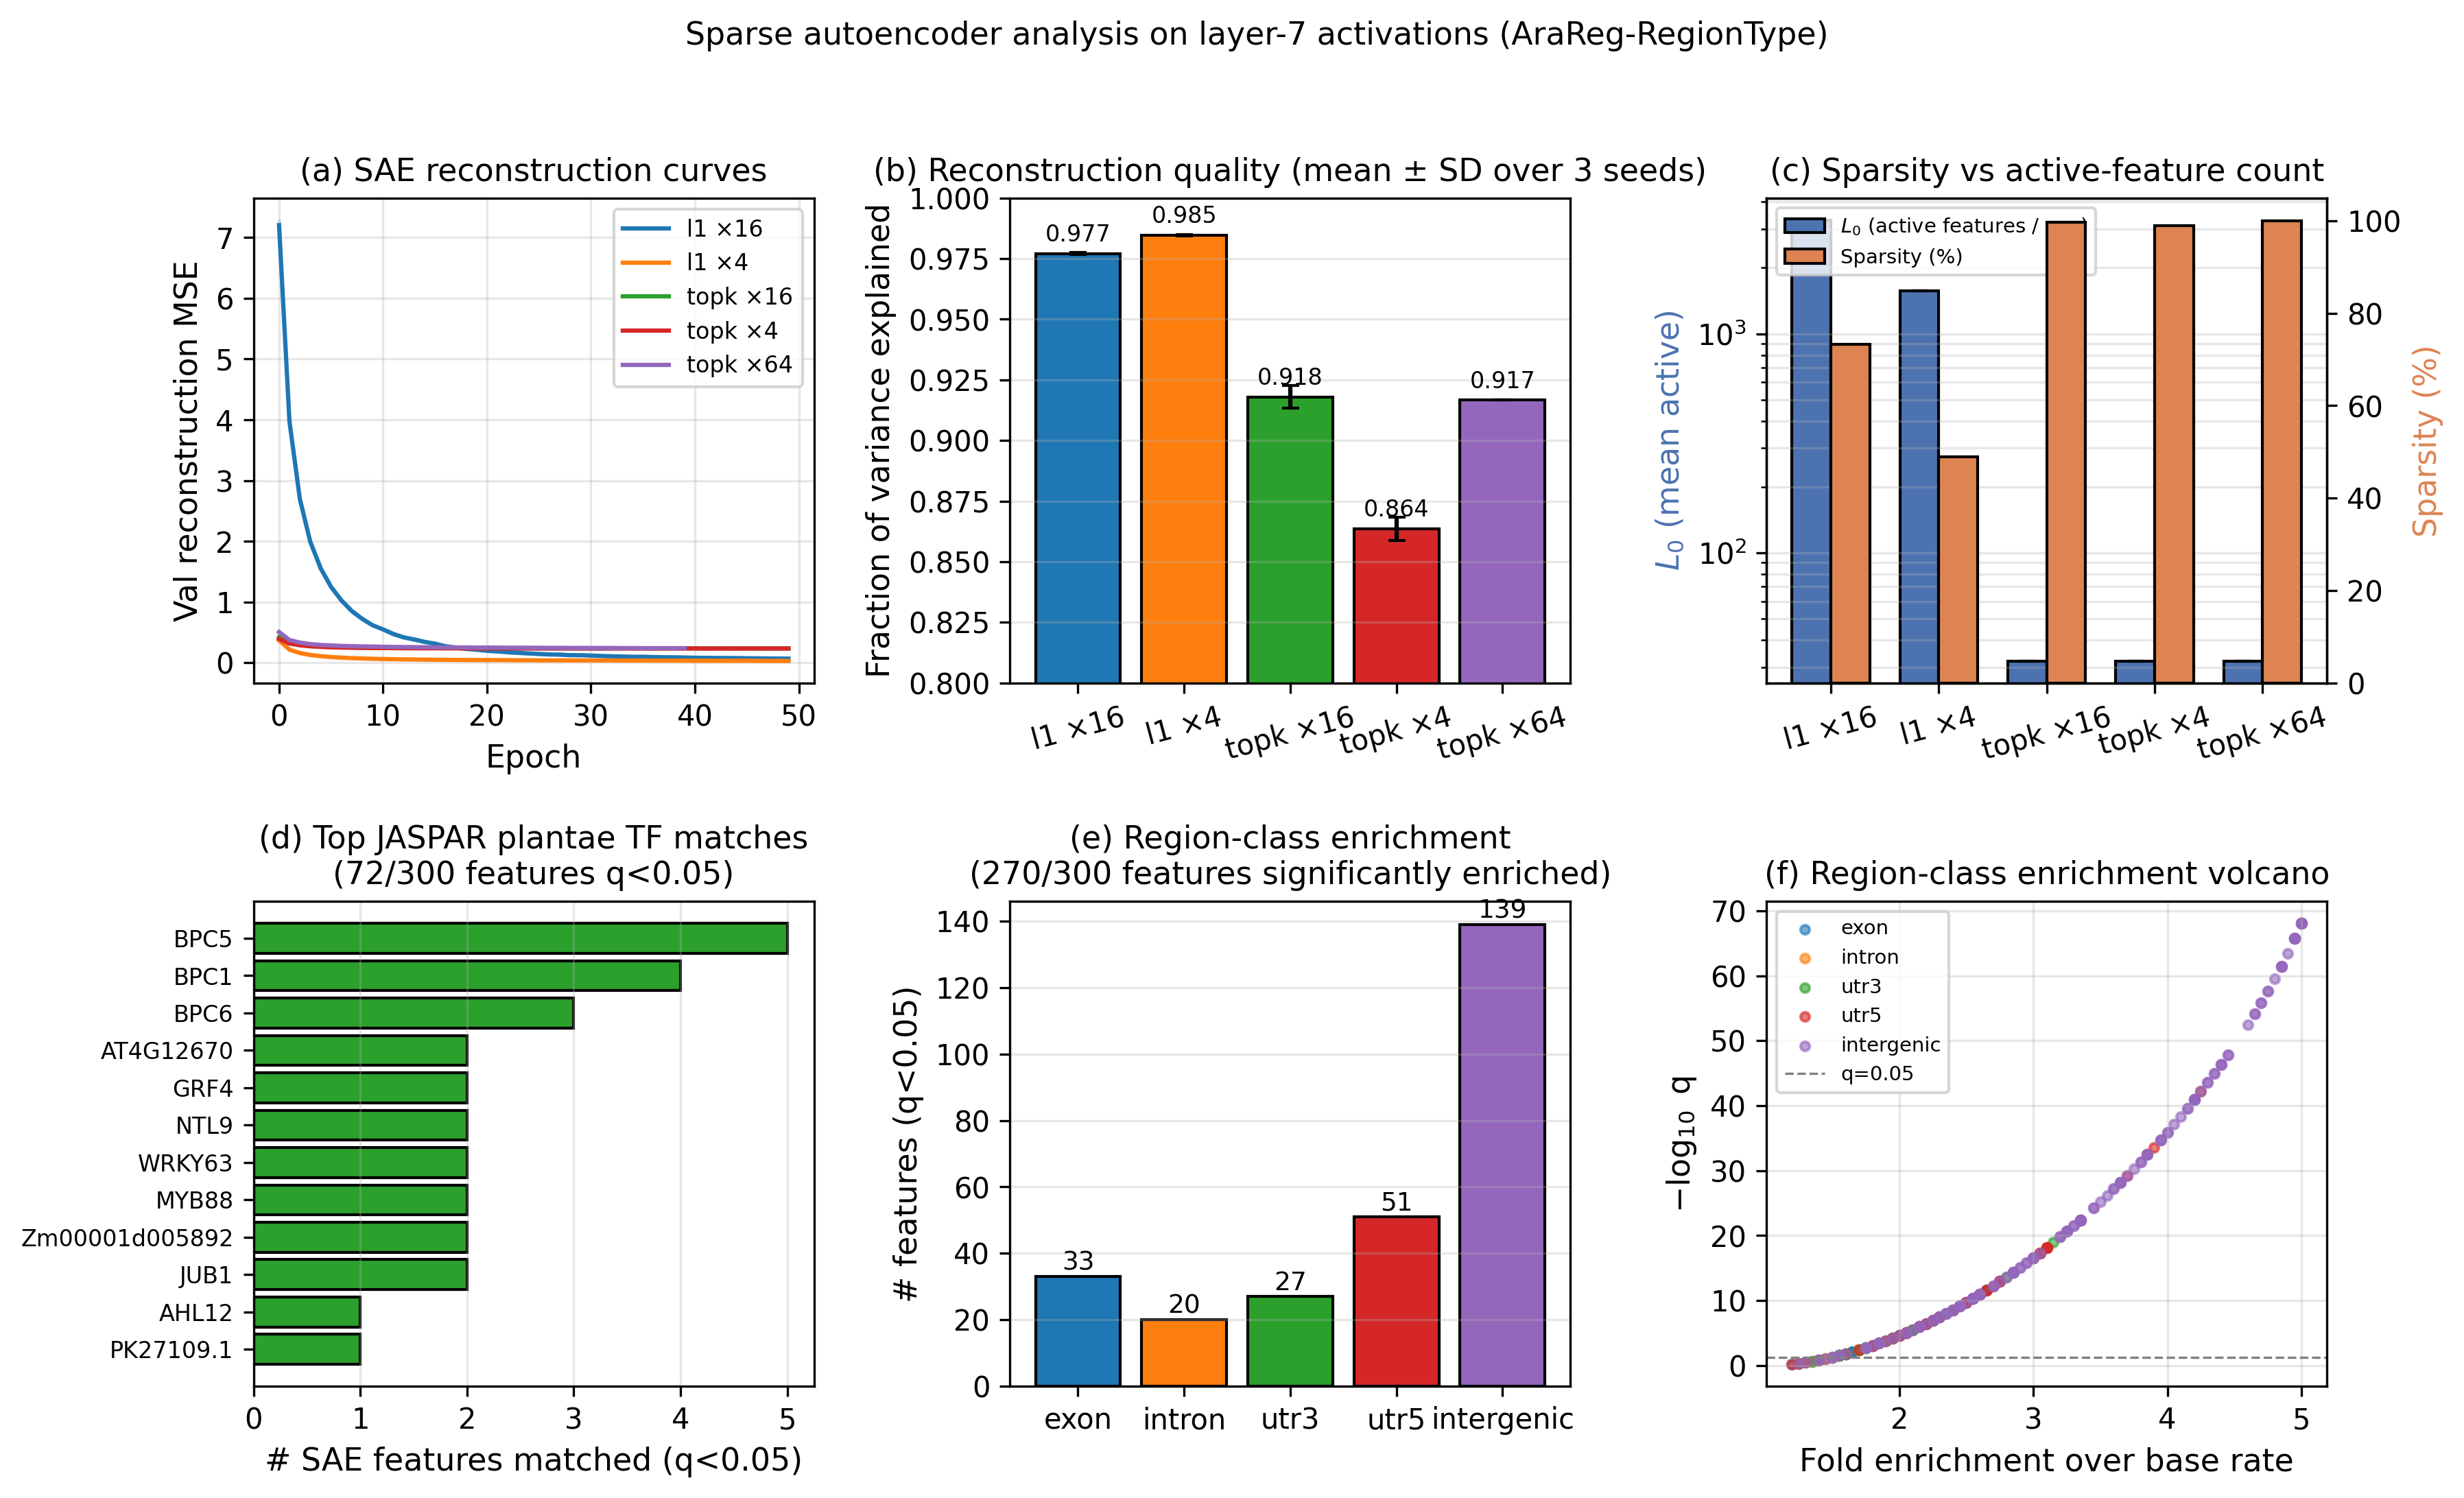
\includegraphics[width=\textwidth]{sae_training.png}
    \caption{\textbf{Sparse-autoencoder analysis on layer-7 activations of
    AraReg-RegionType.} (a)~Validation reconstruction MSE averaged over
    3 seeds per config, shaded $\pm$1~SD. Top-K reaches lower absolute MSE
    than L1 due to different scaling of the reconstruction term.
    (b)~Fraction of variance explained at convergence per config (3-seed
    means; numbers on top).
    (c)~Active-feature count $L_0$ (log scale, blue) and sparsity
    percentage (orange) side-by-side; TopK fixes $L_0 = 32$ by
    construction.
    (d)~Top JASPAR plantae TF families matched by TopK~$\times$~16 SAE
    features (72/300 at BH q$<$0.05); BPC paralogs dominate.
    (e)~Number of features significantly enriched (q$<$0.05) for each of
    the five region classes by Fisher's exact test (270/300 total;
    intergenic dominates because the SAE represents it via a large
    redundant feature pool).
    (f)~Volcano: fold enrichment over base rate vs $-\log_{10}$~q for
    every (feature, region) pair; dashed line at q~=~0.05.}
    \label{fig:sae}
\end{figure}

\paragraph{Motif enrichment.}
\textbf{72 of 300 features (24\%)} have a JASPAR 2024 plantae motif whose
max-score distribution on the feature's top-50 activating sequences is
significantly higher than on a 500-sequence background (Mann--Whitney
one-sided, BH q$<$0.05). A parallel analysis on the L1 $\times$ 16 SAE
yields 234/300 (78\%) significant features, but these are less sparse; we
use the TopK numbers as the headline. Frequent matches cluster by TF
family:
\begin{itemize}[leftmargin=1.4em,topsep=0.2em,itemsep=0.15em]
    \item \textbf{BPC} (BASIC PENTACYSTEINE): BPC5 (5 features), BPC1~(4),
    BPC6~(3). BPC proteins bind GAGA-like repeats and regulate homeotic
    genes~\citep{meister2004high}.
    \item \textbf{DOF} (DNA-binding with one finger): DOF3.6, DOF5.8,
    DOF2.4, which regulate light, seed, and stress
    responses~\citep{yanagisawa2004dof}.
    \item \textbf{MYB}: MYB88, MYB48, core plant TFs for development and
    secondary metabolism.
    \item \textbf{NAC}: NAC010, stress- and senescence-related.
    \item \textbf{ERF}: ERF115, an ethylene response factor.
    \item \textbf{B3}: LEC2 (LEAFY COTYLEDON~2), embryo development.
\end{itemize}
These features are rooted in documented plant regulatory biology and
provide a concrete biological interpretation of what Plant-DnaGemma's
layer-7 representation encodes.

Cross-referencing the 72 significant features with the PlantTFDB~5.0
Arabidopsis TF catalogue~\citep{tian2020plantregmap} assigns 47 to named
plant-TF families: BBR-BPC (12 features), NAC (10), MYB/MYB-related (6),
AT-hook (4), WRKY (4), Dof (3), GRF (2), ERF (2), and single features from
HD-ZIP, B3, SBP, and Trihelix families. The remaining 25 features match
JASPAR motifs that lack a direct Arabidopsis gene-name mapping in
PlantTFDB (often paralogs from rice or maize in JASPAR).

\paragraph{Region-class enrichment.}
In addition to motif matching, for each feature we test whether its
top-100 activating sequences are enriched for a specific region class
using Fisher's exact test with BH FDR. \textbf{270 of 300 features (90\%)}
are significantly enriched for one region class at q$<$0.05. Breakdown:
139 intergenic, 51 UTR5, 33 exon, 27 UTR3, 20 intron. Several features
simultaneously pass both tests --- for example, feature 3617 matches BPC5
(q~=~6$\times$10$^{-6}$) \emph{and} is 85\% UTR5-enriched (fold
4.25$\times$), consistent with BPC5 binding regulatory elements in
upstream regions.

\paragraph{Causal feature ablation.}
For the top-5 region-enriched features per class (25 total), zeroing the
feature in the SAE latent and re-passing the reconstructed activation
through the frozen probe reveals two regimes. Ablating UTR5-enriched
features reduces UTR5 accuracy by 5.6~pp more than it reduces other
classes (mean over 5 features); UTR3-features give targeted 5.5~pp drops
on UTR3 accuracy --- evidence that these features \emph{causally} encode
UTR identity. For exon, intron, and intergenic features the per-class
targeted effect is weaker, because the SAE represents these classes with
many redundant features (33, 20, and 139 respectively) so removing one
makes little difference. Some region classes are encoded by
\emph{monosemantic} SAE features; others by \emph{distributed}
redundant ones.

\subsection*{Activation patching and per-component ablations}
\label{sec:mechanistic}

To address the concern that probing is decodability rather than
mechanism, we run two causal interventions on the splice-site task.

\paragraph{Activation patching.}
For each of 64 real donor and acceptor windows from AraReg-Splice we
construct two corrupted variants: canonical-base corruption (GT$\to$CC at
the splice position), which destroys the motif while preserving
everything else; and a dinucleotide-preserving shuffle of a 40-nt window
centered on the splice site, which preserves local composition but
destroys positional structure. For each layer and direction (denoising:
plug clean activations into the corrupt pass; noising: the reverse) we
measure the effect on a frozen layer-7 logistic probe, normalized by the
clean$\to$corrupt logit gap.

Canonical-base corruption produces large causal damage concentrated in
early-middle layers: a noising effect of $+60$ normalized units at
layer~2 and $+59$ at layer~3, decaying to near zero by layer~6.
Denoising at layers 0--4 recovers $+12$ units --- the splice-site signal
enters at the embedding layer and propagates through the first half of
the stack. Dinucleotide-shuffled corruption at the splice position
produces a smaller damage profile (peak absolute effect 23 units at
layer~2), consistent with the shuffled version preserving enough local
composition to keep the classifier partly functional.

\paragraph{Negative control.}
As a specificity check we repeat the dinucleotide-shuffled corruption at
a random non-motif position (offset $\pm$150\,nt from the splice site).
The peak absolute effect drops from 23 units (splice-centered) to 11
units (random-position) at layer~3 --- roughly half the magnitude. The
splice-site position itself is therefore causally important, not merely
any corrupted 40-nt window.

\paragraph{Head and MLP ablations.}
Zeroing each of the $12 \times 12 = 144$ attention heads (via its
output-projection contribution) and each of the 12 MLP blocks and
remeasuring the frozen layer-7 splice-classifier accuracy on a balanced
120-sequence held-out-chromosome subset (baseline 64.2\%) gives a
striking result (Figure~\ref{fig:head-ablations}):

\begin{figure}[t]
    \centering
    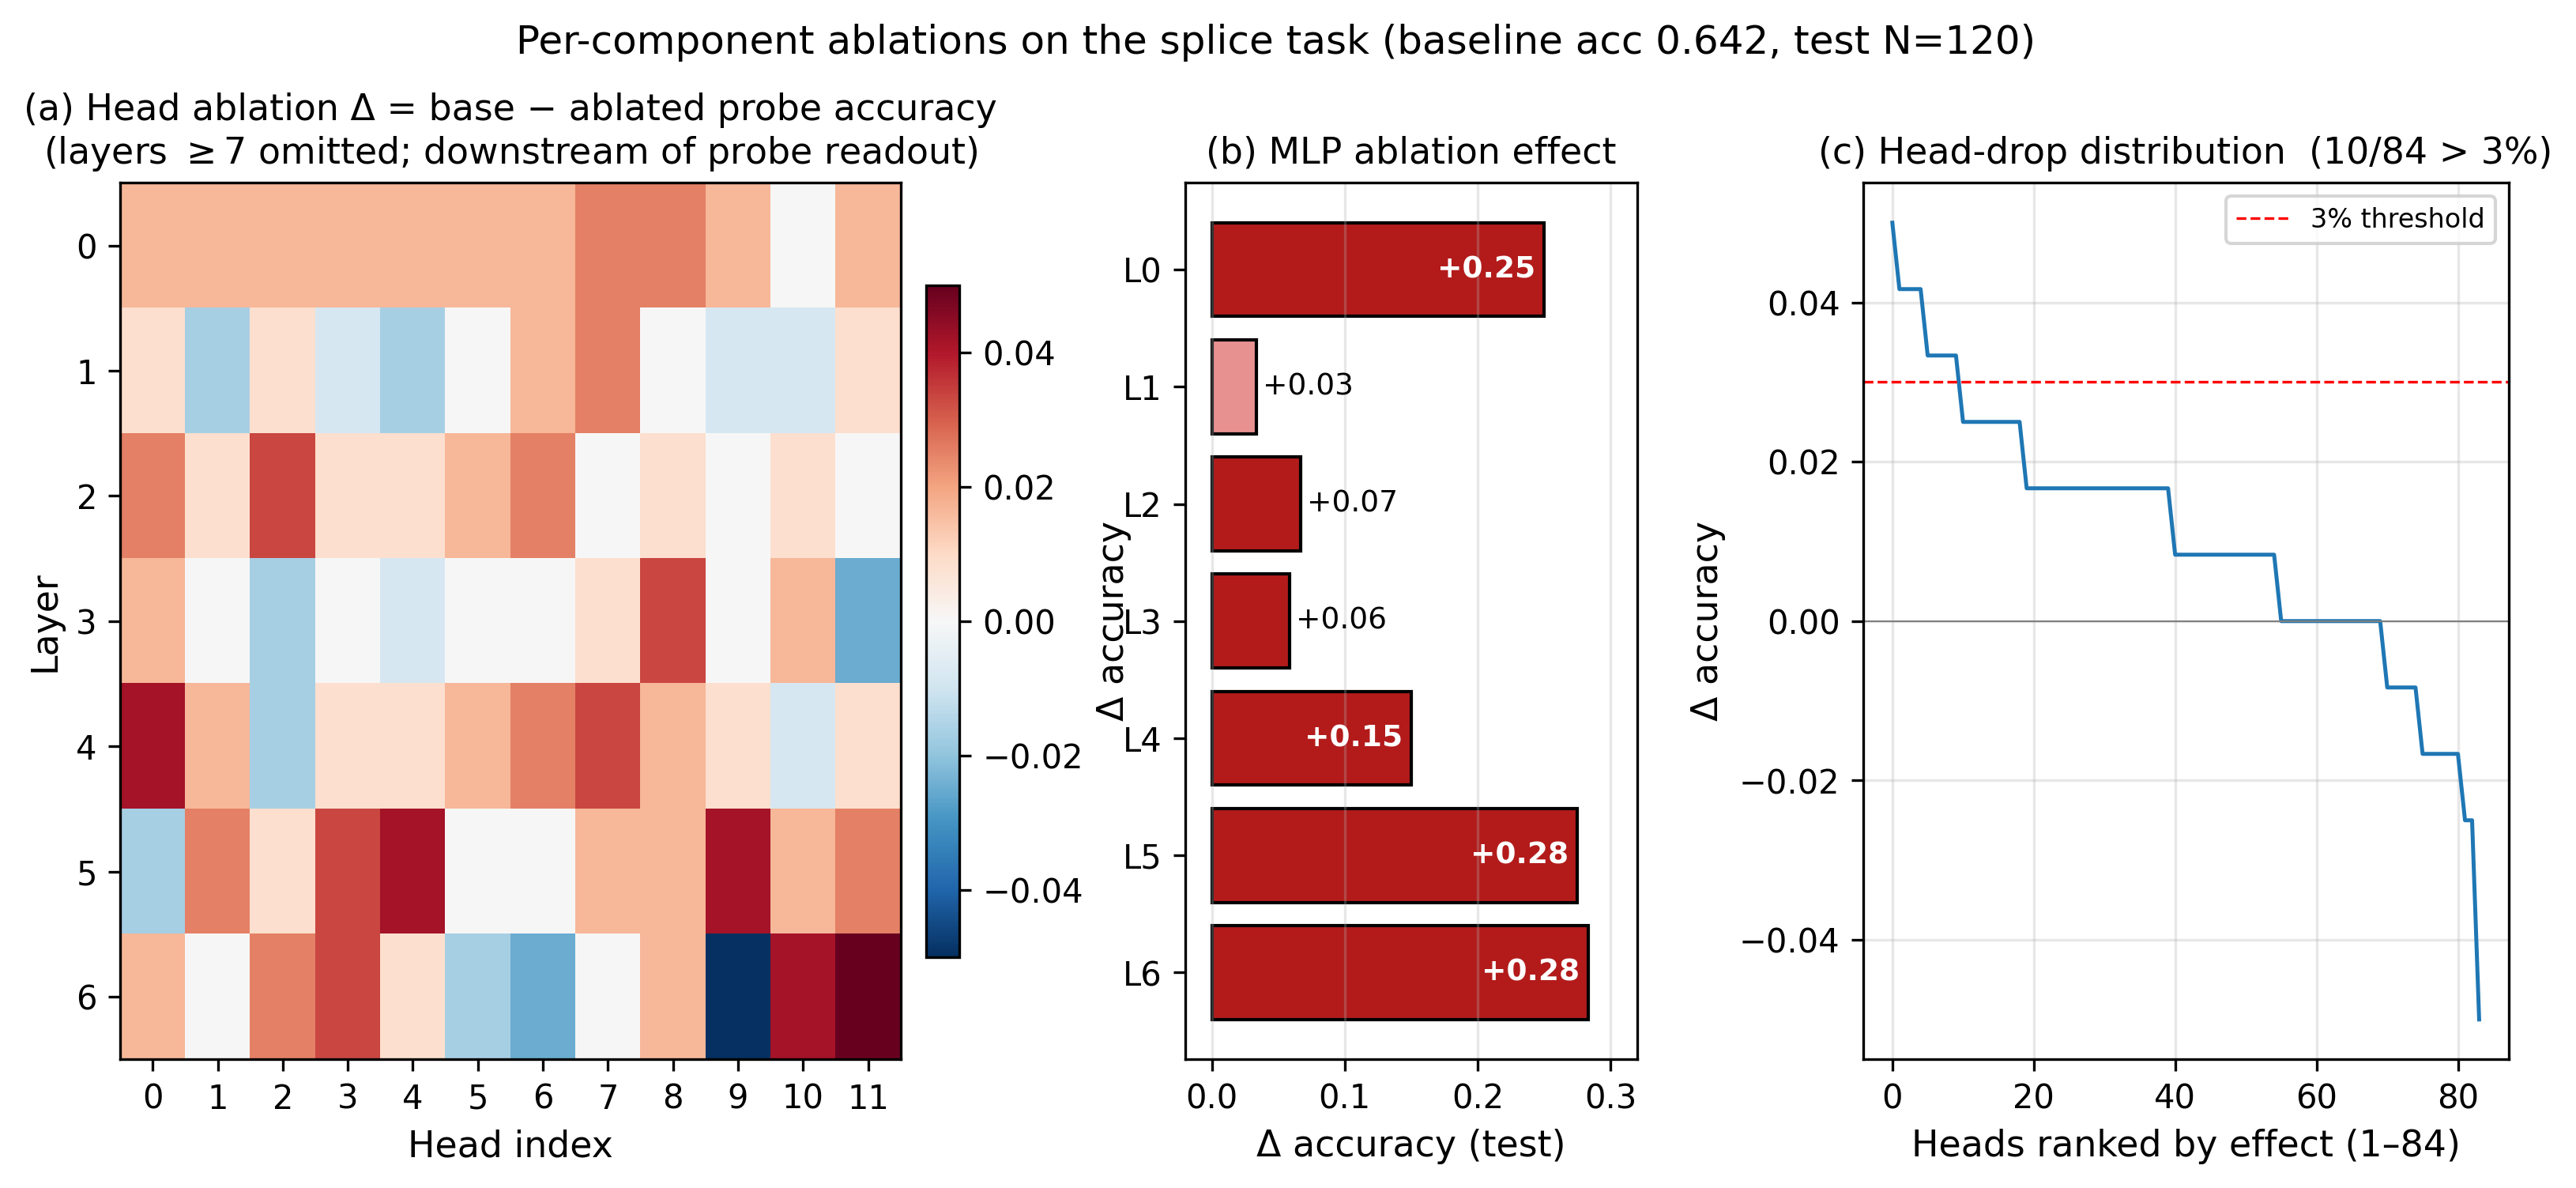
\includegraphics[width=\textwidth]{head_ablations_splice.png}
    \caption{\textbf{Per-component ablations on the splice task}
    (baseline test accuracy 0.642 on 120 held-out-chromosome sequences).
    (a)~Head-ablation $\Delta$ accuracy per (layer, head); layers
    $\geq$~7 are omitted because they sit downstream of the layer-7 probe
    readout. (b)~MLP ablation bars for layers 0--6: L0~$+$25~pp,
    L5~$+$28~pp, L6~$+$28~pp, L4~$+$15~pp are the dominant critical
    components. (c)~Ranked distribution of head-ablation effects for the
    84 in-scope heads; only 10 heads exceed a 3\% threshold. Attention is
    distributed and redundant; MLPs carry the causal load.}
    \label{fig:head-ablations}
\end{figure}

\begin{itemize}[leftmargin=1.4em,topsep=0.2em,itemsep=0.15em]
    \item \textbf{Individual attention heads are largely redundant}: mean
    accuracy drop across all 144 heads is 0.6\%, maximum 5.0\% (L6H11).
    Only 10 of 144 heads produce a drop exceeding 3\%. No single head is
    a ``splice detector'' circuit.
    \item \textbf{MLPs are causally critical}: zeroing the MLP at
    layer~6 drops accuracy by 28.3~pp (from 64.2\% to 35.8\%); layer 5's
    MLP drop is 27.5~pp; layer 0's is 25.0~pp; layer 4's is 15.0~pp.
    Ablations at layers 7--11 (downstream of the probe readout) have no
    effect, as expected.
\end{itemize}

This is a genuinely mechanistic rather than descriptive finding: splice-
site processing is routed primarily through early-middle MLP blocks,
with attention providing distributed, redundant routing. This differs
from the pattern seen in NLP circuit-discovery
work~\citep{wang2023interpretability, olsson2022context}, where a small
number of attention heads are often individually critical.

\section*{Discussion}
\label{sec:discussion}

\paragraph{What pretraining learns.}
Plant-DnaGemma's probing advantages (+6.9~pp over the best learned
baseline on 5-way region-type, +3.4~pp on 3-way splice, +11.7~pp over the
4-mer logistic on GC-matched 4-way species) are modest: real genomic
sequences embed rich compositional information (splice-site consensus,
codon bias, regulatory-element frequency) that simple $k$-mer or CNN
baselines partially recover. That a 152M-parameter foundation model
still beats learned baselines \emph{trained with the task labels} on the
multi-class tasks demonstrates that pretraining supplies features not
reachable from task-supervised training alone. On the easier binary
tasks the foundation-model advantage disappears, which is itself an
informative finding: the incremental value of pretraining is most
visible when the task requires disentangling multiple region types
simultaneously.

\paragraph{Distributed, yet grounded, representations.}
The SAE analysis provides a feature-level grounding of Plant-DnaGemma:
24\% of the top-300 features (72 of 300) have a significant JASPAR
plantae TF-motif match, with 47 mapping to named PlantTFDB Arabidopsis
TF families. The BPC enrichment (12/72 features map to BBR-BPC family
members) is biologically sensible: BPC factors bind GAGA-like
repeats~\citep{meister2004high}, a form of compositional regularity that
Plant-DnaGemma's BPE tokenization and heavy-tailed SAE activation
distribution are well suited to capture. Scaling to $64\times$ expansion
at fixed $K{=}32$ yields \emph{no} additional variance-explained gain
over $16\times$ and produces 32\% dead features, suggesting that at
this per-sample activation budget the dictionary is already saturated;
an honest scaling assessment would require increasing $K$ alongside
$d_h$. Directed feature ablation validates the interpretation for UTR-
enriched features (see the monosemantic vs distributed contrast above);
feature steering is left to future work.

\paragraph{Phylogeny, once GC is controlled.}
At the scale of 6 species $\times$ 2\,000 windows with GC-matched and
partial-Mantel controls, Plant-DnaGemma does encode phylogenetic
structure beyond GC: 68\% accuracy (chance 25\%) on the GC-matched
4-species task and partial Mantel r~=~0.55 (p~=~0.019) are both
statistically significant non-compositional signals. This signal
requires both sufficient sample size and window length to detect: at a
few hundred short windows it is obscured by the GC confound.

\paragraph{Limitations.}
\label{sec:limitations}
(1)~\emph{Pretraining--evaluation overlap}: Plant-DnaGemma was trained on
plant genomes including Arabidopsis, so AraReg evaluation benefits from
pretraining familiarity. We partially control for this via the held-out
tomato/soybean analysis.
(2)~\emph{Model scope}: we study a single model; extension to AgroNT and
PlantCAD2 is left for future work.
(3)~\emph{SAE scale}: our $64\times$ expansion at $d_h = 49\,152$ is
modest compared to $256\times$ in contemporary NLP SAE work, but the
plateau between $16\times$ and $64\times$ suggests larger dictionaries
are unlikely to reveal qualitatively new features at fixed $K = 32$.
(4)~\emph{Motif enrichment}: PWM scoring against JASPAR is coarse; de
novo motif discovery with STREME/TomTom would yield finer-grained
matches.
(5)~\emph{1-NN held-out clade}: tomato and soybean are GC-close to
Arabidopsis (0.34--0.36) and GC-distant from the monocots (0.44--0.47),
so part of the clade clustering we observe could be GC-driven; the
partial Mantel test, which controls for GC, is the more conservative
piece of phylogenetic evidence.
(6)~\emph{Activation patching} uses a frozen layer-7 probe as metric;
path patching into individual heads~\citep{wang2023interpretability} is
deferred to future work.

\section*{Conclusions}
\label{sec:conclusions}

We have presented a reproducible methodology for the mechanistic
interpretability of plant genomic foundation models, instantiated on
Plant-DnaGemma. The protocol integrates annotated plant-bioinformatics
resources (TAIR10, Araport11, EPDnew, Ensembl Plants, JASPAR plantae,
PlantTFDB) with modern interpretability tooling (probing with learned
baselines, GC-matched composition controls, phylogenetic residualization,
sparse autoencoders, causal per-component ablations). On 5-way
region-type and 3-way splice-site classification Plant-DnaGemma
outperforms $k$-mer logistic regression, CNN, bi-LSTM, and $k$-mer-MLP
baselines; on simpler binary tasks a task-supervised CNN effectively
matches the foundation model. On cross-species representation the model
captures non-compositional phylogenetic structure visible through a
GC-matched probe and a partial Mantel test. A Top-K sparse autoencoder's
layer-7 features ground to documented plant transcription-factor motifs
for 24\% of the top-300 features, with PlantTFDB family assignments for
47 of these 72 matches. Per-component ablations on splice-site
processing show that the causal load is carried by early-middle MLPs,
not by individual attention heads. Together these results provide both
an evaluation protocol --- directly reusable for any plant genomic
foundation model --- and an initial mechanistic picture of what
Plant-DnaGemma has learned.

\section*{List of abbreviations}
\noindent AUC, area under the receiver-operating-characteristic curve;
BH, Benjamini--Hochberg;
BPC, Basic Pentacysteine;
BPE, Byte-Pair Encoding;
CKA, Centered Kernel Alignment;
CNN, Convolutional Neural Network;
CV, cross-validation;
DOF, DNA-binding with One Finger;
ECE, Expected Calibration Error;
EPD, Eukaryotic Promoter Database;
ERF, Ethylene Response Factor;
GC, guanine--cytosine content;
JASPAR, open-access database of TF binding profiles;
MLP, Multi-Layer Perceptron;
MYB, Myeloblastosis TF family;
NAC, NAM/ATAF/CUC TF family;
OVR, one-versus-rest;
PWM, Position Weight Matrix;
SAE, Sparse Autoencoder;
TAIR, The Arabidopsis Information Resource;
TF, Transcription Factor;
TFBS, TF Binding Site;
TSS, Transcription Start Site;
WRKY, WRKY TF family.

\section*{Declarations}

\paragraph{Ethics approval and consent to participate.}
Not applicable. This study uses only publicly available genomic data; no
animal or human subjects were involved.

\paragraph{Consent for publication.}
Not applicable.

\paragraph{Availability of data and materials.}
All analysis code, data-preparation scripts, frozen train/val/test
splits, intermediate JSON result files, and figure-generation scripts
are publicly available at
\url{https://github.com/Biodyn-AI/aido-mechinterp}. A tagged snapshot of
the repository together with the trained sparse-autoencoder weights,
pre-computed motif-score matrices, and built parquet datasets is
deposited at Zenodo:
\url{https://doi.org/10.5281/zenodo.18665058}.
Source datasets are pinned to the following public versions, with
download scripts provided: TAIR10 genome and Araport11 annotations
(Ensembl Plants release~58); EPDnew \textit{A.~thaliana} promoter
database (v1); JASPAR 2024 CORE \textit{plantae} non-redundant PFMs;
PlantTFDB~5.0 Arabidopsis TF list. Stochastic pipelines use fixed
seeds (0,~1,~2).

\paragraph{Competing interests.}
The authors declare that they have no competing interests.

\paragraph{Funding.}
This work received no specific grant from any funding agency in the
public, commercial, or not-for-profit sectors.

\paragraph{Authors' contributions.}
IK is the sole author and conceived the study, designed and ran all
experiments, analyzed the results, and wrote the manuscript. The author
read and approved the final manuscript.

\paragraph{Acknowledgements.}
Not applicable.

\bibliography{references}

\end{document}
